\documentclass[a4paper,12pt,fleqn]{article}%fleqn pour aligner les equations à gauche
\usepackage{../../Styles/Cours}

\newcommand{\chnum}{Chapitre 6}
\newcommand{\chtitle}{Le son émis par une corde vibrante}
\newcommand{\dtype}{Activité}

\begin{document}
\maketitle
\begin{figure}[h!]
    \caption{Instruments à corde}
    \label{doc1}
    \begin{minipage}{.48\linewidth}
        Une guitare comporte six cordes tendues, de masse linéique (épaisseurs) différentes, que l'on peut faire vibrer. Les fréquences des notes que l'on peut jouer sont différentes :
        \begin{itemize}
            \item La fréquence de la note produite par la vibration d'une corde dépend de son épaisseur et de sa tension $T$. En tournant une clé, le guitariste tend plus ou moins chacune des cordes et modifie la fréquence de la note.
            \item Le guitariste peut modifier la longueur des cordes en les pinçant et ainsi faire varier la fréquence de son émis.
        \end{itemize}
        Dans le cas des instruments à vent, c'est la vibration d'une colonne d'air qui permet d'émission d'un son. Ainsi, la fréquence est associée à la longueur de la colonne d'air.
    \end{minipage}\hspace{1em}
    \begin{minipage}{.48\linewidth}
        La masse linéique est une grandeur notée $\mu$ et exprimée en \unit{\kilo\gram\per\meter} qui correspond à la masse $m$ de la corde par unité de longueur $l$. Elle peut donc être calculée comme étant $\mu = \dfrac{m}{l}$.
        \begin{center}
            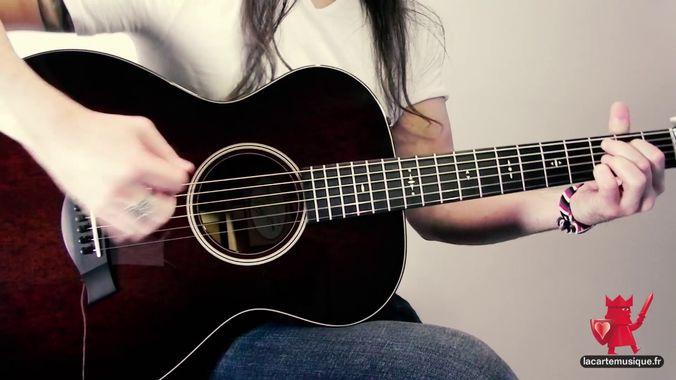
\includegraphics[width=\linewidth]{1ES_C6_Act2_Fig1.jpg}
        \end{center}
    \end{minipage}
\end{figure}

\begin{figure}[h!]
    \caption{physique des cordes}
    \label{doc2}
    \begin{minipage}{.48\linewidth}
       Le physicien allemand, Franz Melde a travaillé sur les ondes acoustiques. En fixant une corde à ses deux extrémités, il observe que s'il la fait vibrer avec certaines valeur de fréquences, la corde forme un ou plusieurs fuseaux de grande amplitude : elle entre en raisonnance.\\
       Il découvre alors que la fréquence fondamentale du son émis correspond à la fréquence  pour laquelle la corde vibre en ne formant qu'un seul fuseau.\\
       Mais la corde peut présenter plusieurs fuseaux. Dans le cas de deux fuseaux, la fréquence avec laquelle la corde vibre est appellée première harmonique. La fréquence permettant d'observer trois fuseaux est la seconde harmonique et ainsi de suite.
    \end{minipage}\hspace{1em}
    \begin{minipage}{.48\linewidth}
        \begin{center}
            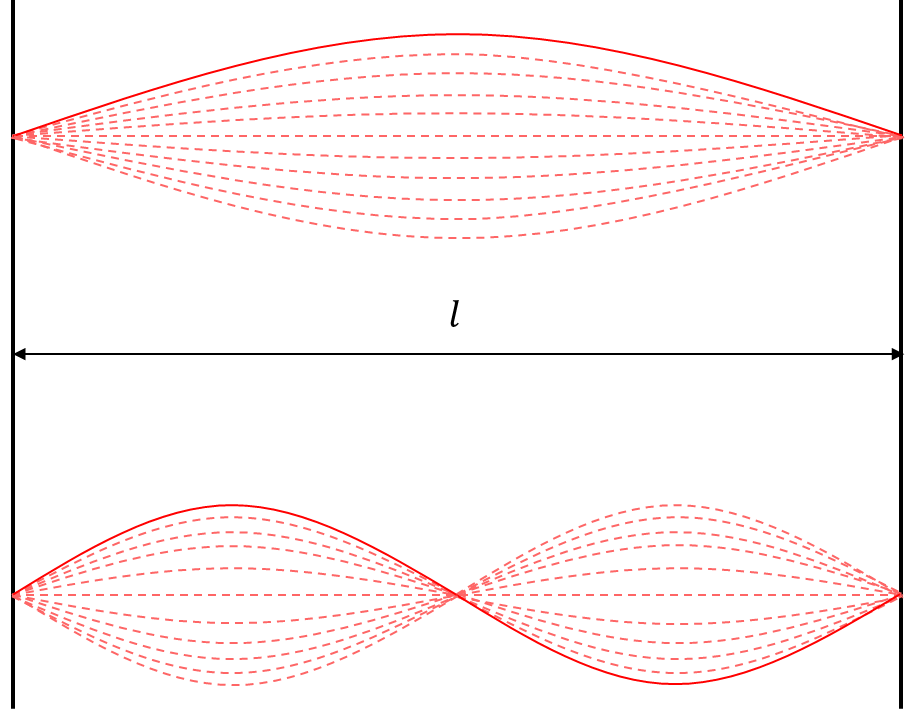
\includegraphics[width=\linewidth]{1ES_C6_Act3_Fig2.png}
        \end{center}
    \end{minipage}
\end{figure}

\begin{figure}[h!]
    \caption{Expérience}
    \label{doc3}
    \begin{minipage}{.48\linewidth}
       Les extrémités d'une corde sont reliées d'une part à un vibreur alimenté par un générateur basse fréquence (GBF) et d'autre part à une masse de \SI{50}{g} par l'intermédiaire d'une poulie. La corde est réglée à une longueur (entre le  vibreur et la poulie) de \SI{50}{cm}. On fait varier la fréquence du GBF jusqu'à ce que la corde vibre en ne formant qu'un seul fuseau avec une amplitude maximale. La fréquence $f_1$ correspondante est notée. On continue à faire varier la  fréquence du GBF jusqu'à obtenir les fréquences $f_2$ et $f_3$. Puis on renouvelle toute l'expérience avec une longueur de corde de \SI{1}{m}. Les résultats de l'expérience sont donnés dans le tableau ci-contre.
    \end{minipage}\hspace{1em}
    \begin{minipage}{.48\linewidth}
        \begin{tabular}{>\centering m{.25\linewidth}|>\centering m{.1\linewidth}|>\centering m{.1\linewidth}|>\centering m{.1\linewidth}|>\centering m{.1\linewidth}|>{\centering \arraybackslash} m{.1\linewidth}}
            \hline
            \textbf{Longueur $l$ de la corde (en \unit{\meter})} & 0,50 & 0,50 & 0,50 & 1,00 & 1,00\\
            \hline
            \textbf{Fréquence (en \unit{\hertz})} & 80 & 160 & 240 & 40 & 80\\
            \hline
            \textbf{Nombre de fuseaux} & 1 & 2 & 3 & 1 & 2 \\
            \hline
        \end{tabular}
    \end{minipage}
\end{figure}

\begin{figure}[h!]
    \caption*{Formule :}
    La fréquence fondamentale, notée $f_1$, du son émis par une corde vibrante de longueur $l$ est donnée par la relation : $$f_1 = \dfrac{1}{2\times l}\times \sqrt{\dfrac{T}{\mu}}$$
\end{figure}

\newpage
\textbf{Questions :}
\begin{enumerate}
    \item Comment évolue la fréquence du son émis par une guitare si on tend d'avantage la corde jouée ? Justifier. (Doc.~\ref{doc1} et~\ref{doc2})
    \item De quels paramètres la fréquence fondamentale du son émis par une corde dépend-elle ? (Doc.~\ref{doc1} et~\ref{doc2})
    \item Quel phénomène se produit dans les instruments à vent ? De quels paramètres la fréquence du son émis dépend-elle ? (Doc.~\ref{doc1})
    \item Quelle est la valeur de la fréquence fondamentale du son émis par la corde de \SI{50}{cm} ? (Doc.~\ref{doc3})
    \item Pour une même longueur de corde, quelle relation existe-t-il entre les valeurs de la fréquence fondamentale et celles des harmoniques ? (Doc.~\ref{doc3})
    \item Expliquer comment prévoir théoriquement la valeur de la fondamentale mesurée avec une corde de \SI{25}{cm}.
    \item Quelle est l'influence de la longueur de la corde sur la fréquence fondamentale du son émis ? (Doc.~\ref{doc3})
    \item Comment peut-on expliquer le fait que les sons émis par les cordes d'une contrebasse soient plus graves que ceux émis par les cordes d'un violon ?
\end{enumerate}
\end{document}